\chapter{Modelul ARMA}

\section{Scopul metodei}

Putem folosi această metodă pentru a prezice următoarele puncte dintr-o serie de timp, cu o acurateţe ce în mod natural va scădea
cu cât încercăm să vedem mai mult în viitor, şi astfel putem să semnalăm o posibilă anomalie dacă noul eşantion pe care credem că îl vom obţine şi în realitate, deviază cu mult faţă de punctele înregistrate deja.

Pentru a decide dacă un nou punct este sau nu anomalie, vom folosi un prag care este influenţat într-o proporţie majoră de volatilitatea instrumentului, anume indicatorul beta despre care am vorbit în 
introducere.

Acest model funcţionează bine atunci când datele din viitor pot fi modelate cu ajutorul datelor din trecut. Dacă nu există nicio relaţie între
evenimentele din trecut şi cele din viitor, atunci modelul nu va putea extrage caracteristicile necesare prezicerii.

\section{Ideea din spatele metodei}

Acest model este compus din 2 părţi, AR(AutoRegressive) şi MA(Moving-Average).

Partea autoregresivă încearcă sa modeleze punctele din seria de timp folosind o regresie liniară bazată pe un număr finit de puncte din trecut
la care se adaugă şi o variabilă de eroare care se poate presupune că este independent şi identic distribuită, provenită dintr-o distribuţie Gaussiană. Numărul de puncte din trecut este notat cu $p$ şi reprezintă singurul hiperparametru pentru această componentă.

Partea de medie glisantă încearcă să modeleze termenul eroare folosind o combinaţie liniară dintr-un număr de termeni de eroare din trecut. Despre aceste erori, putem face aceleaşi presupuneri ca mai sus. Numărul de termeni eroare din trecut este notat cu $q$ şi reprezintă
hiperparametrul pentru această componentă.

Aceste 2 componente sunt însumate pentru a obţine modelul final pe care îl vom putea folosi pentru a prezice noile puncte din seria de timp.

Găsirea hiperparamterilor optimi se poate realiza cu ajutorul funcţiei de autocorelaţie parţială pentru aflarea lui $p$, iar pentru $q$ putem folosi
functia de autocorelaţie. Apoi, pentru rezolvarea sistemului rezultat se poate folosi tehnica celor mai mici pătrate.

\section{Reprezentarea matematică}

ARMA(p, q):
\[
X_t = \varepsilon_t + \sum_{i=1}^{p} \phi_i X_{t-i} + \sum_{j=1}^{q} \theta_j \varepsilon_{t-j}
\]

AR(p):
\[
X_t = \varepsilon_t + \sum_{i=1}^{p} \phi_i X_{t-i} 
\]

MA(q):
\[
X_t = \mu + \varepsilon_t + \sum_{j=1}^{q} \theta_j \varepsilon_{t-j}
\]

unde $X_t$ este seria de timp, $\varepsilon_t$ este termenul eroare, $\mu$ este media semnalului $X_t$ pe care o presupunem 0 de obicei, iar 
$\phi_i$ şi $\theta_j$ sunt parametrii pentru regresia liniară a modelului AR, respectiv pentru combinaţia liniară a modelului MA.

\section{Implementare}

\noindent Metoda ARMA se implementează în python cu ajutorul funcției ARIMA din $statsmodels$. Ținând cont că ARMA(p,q) = ARIMA(order=(p,0,q)), se stabilește $p$ la o zecime din lungimea seriei de timp și un prag superior pentru $q$ ($qmax$, probabil 5 pentru că ARIMA rulează lent).\\
Se construiește modelul ARMA(p,q) pentru fiecare q de la 1 la $qmax$ și se prezice următoarea valoare a seriei. Media valorilor obținute reprezintă predicția.\\
Dacă modulul diferenței dintre valoarea reală a seriei și predicție depășeste un anumit prag, se consideră anomalie.\\
Pragul se stabilește în funcție de predicțiile obținute pentru fiecare valoare a lui q.\\
\\
\textbf{Aplicare pentru ultima valoare a seriei}\\
Modelul ARMA se construiește pentru toată seria înafară de ultima valoare sau pe ultimele $k$\% valori înafară de ultima. Se aplică pașii anteriori pentru ultima valoare a seriei.\\
\\
\textbf{Aplicare pe seria generală}\\
Pentru fiecare $start$ de la 2$p$ până la $n-1$ se aplică același algoritm ca la aplicarea pentru ultima valoare a seriei trunchiate până la $start$, cu diferența că pragul care indică anomeliile poate fi setat ulterior dacă se cunoaște dinainte procentul de anomalii din serie.\\
\textbf{Exemplu de rulare}\\
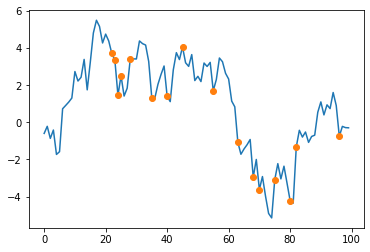
\includegraphics[width=\linewidth]{ARMA.png}